\documentclass[11pt,a4paper]{article}
\usepackage[margin=2.2cm]{geometry}
\usepackage{graphicx,booktabs,amsmath,siunitx,xcolor,tabularx,enumitem,array}
\usepackage[version=4]{mhchem}
\usepackage[most]{tcolorbox}
\usepackage[hidelinks]{hyperref}
\graphicspath{{figures/}}
\setlist{itemsep=2pt,topsep=4pt}
\sisetup{detect-all}

\newtcolorbox{learn}{colback=blue!4,colframe=blue!50!black,boxrule=0.6pt,arc=2pt,
  left=6pt,right=6pt,top=4pt,bottom=4pt,fonttitle=\bfseries,title=Concept to master}
\newtcolorbox{finding}{colback=green!5,colframe=green!40!black,boxrule=0.6pt,arc=2pt,
  left=6pt,right=6pt,top=4pt,bottom=4pt,fonttitle=\bfseries,title=Key finding}
\newtcolorbox{caveat}{colback=red!4,colframe=red!55!black,boxrule=0.6pt,arc=2pt,
  left=6pt,right=6pt,top=4pt,bottom=4pt,fonttitle=\bfseries,title=Caveat / open issue}

\title{\textbf{photocatalyst-dft: where the project stands}\\[4pt]
\large A walkthrough of the Claude Science work, with the concepts behind each step}
\author{Prepared for Lindejiade}
\date{24 October 2026 --- based on the repository state on this date}

\begin{document}
\maketitle

\noindent\textbf{Status in one paragraph.} The molecular half of the project is built and mostly
validated. Sixteen organic photocatalysts are catalogued, cross-checked against PubChem, embedded
in 3D and given B3LYP/def2-SVP frontier orbitals in implicit water. Six molecules have full DFT
geometry optimisations. The three most recent (eosin~Y$^{2-}$, riboflavin, rhodamine~B$^+$) showed
that the MMFF force-field geometries are \emph{not} close to DFT for flexible or charged dyes
(heavy-atom RMSD 0.17--0.40~\AA, versus $\le$0.03~\AA\ for rigid molecules). A new step-5 script
was written to test whether this matters for the orbital energies, but it cannot run yet, because
step~3 has not been rerun on the new geometries. TDDFT and all solid-state work (Week~2) have not
started.

\tableofcontents

%=============================================================================
\section{Project map}

The pipeline is five scripts. Each one reads the previous step's files and writes its own, so any
step can be rerun on its own.

\begin{center}\small
\begin{tabularx}{\linewidth}{@{}l>{\raggedright}p{3.6cm}X@{}}
\toprule
Step & Script & What it does $\to$ main output \\
\midrule
1 & \texttt{01\_represent.py} & SMILES $\to$ checks $\to$ multi-conformer 3D (ETKDGv3 + MMFF94s) $\to$
  \texttt{molecules/xyz/*.xyz}, 2D grid, 3D HTML viewer \\
2 & \texttt{02\_optimize.py} & DFT geometry optimisation (PySCF + geomeTRIC) $\to$
  \texttt{molecules/xyz\_opt/*.xyz}, \texttt{geomopt\_summary.csv} \\
3 & \texttt{03\_frontier.py} & DFT single point on the best available geometry $\to$ HOMO/LUMO
  for all 16, \texttt{frontier\_orbitals.csv}, energy-level diagram \\
4 & \texttt{04\_orbitals.py} & Orbital cube files + fragment localisation (Mulliken) $\to$
  \texttt{orbital\_localization.csv}, isosurface figure \\
5 & \texttt{05\_geometry\_check.py} & \textbf{New.} Does the geometry (MMFF vs DFT) change the
  orbital energies? $\to$ \texttt{geometry\_sensitivity.csv} (\emph{not yet produced}) \\
\midrule
--- & \texttt{utils/common.py} & Shared code: xyz read/write, building the PySCF molecule, the DFT
  settings, constants, plotting style \\
\bottomrule
\end{tabularx}
\end{center}

\noindent The level of theory is the same everywhere: \textbf{B3LYP/def2-SVP, density fitting,
ddCOSMO water ($\varepsilon = 78.36$), restricted closed shell, no dispersion correction.}

%=============================================================================
\section{Step 1 --- Catalogue and molecular representation}

\subsection{The catalogue}
\texttt{data/organic\_photocatalysts.csv} has one row per molecule and 20 columns. The ones the
code depends on are \texttt{slug} (the file-name ID used by every later step), \texttt{smiles},
\texttt{formula}, \texttt{charge} and \texttt{inchikey}. The rest is literature metadata: family,
role, $\lambda_\text{max}$, the lowest absorption band and redox notes.

\begin{figure}[h]
\centering
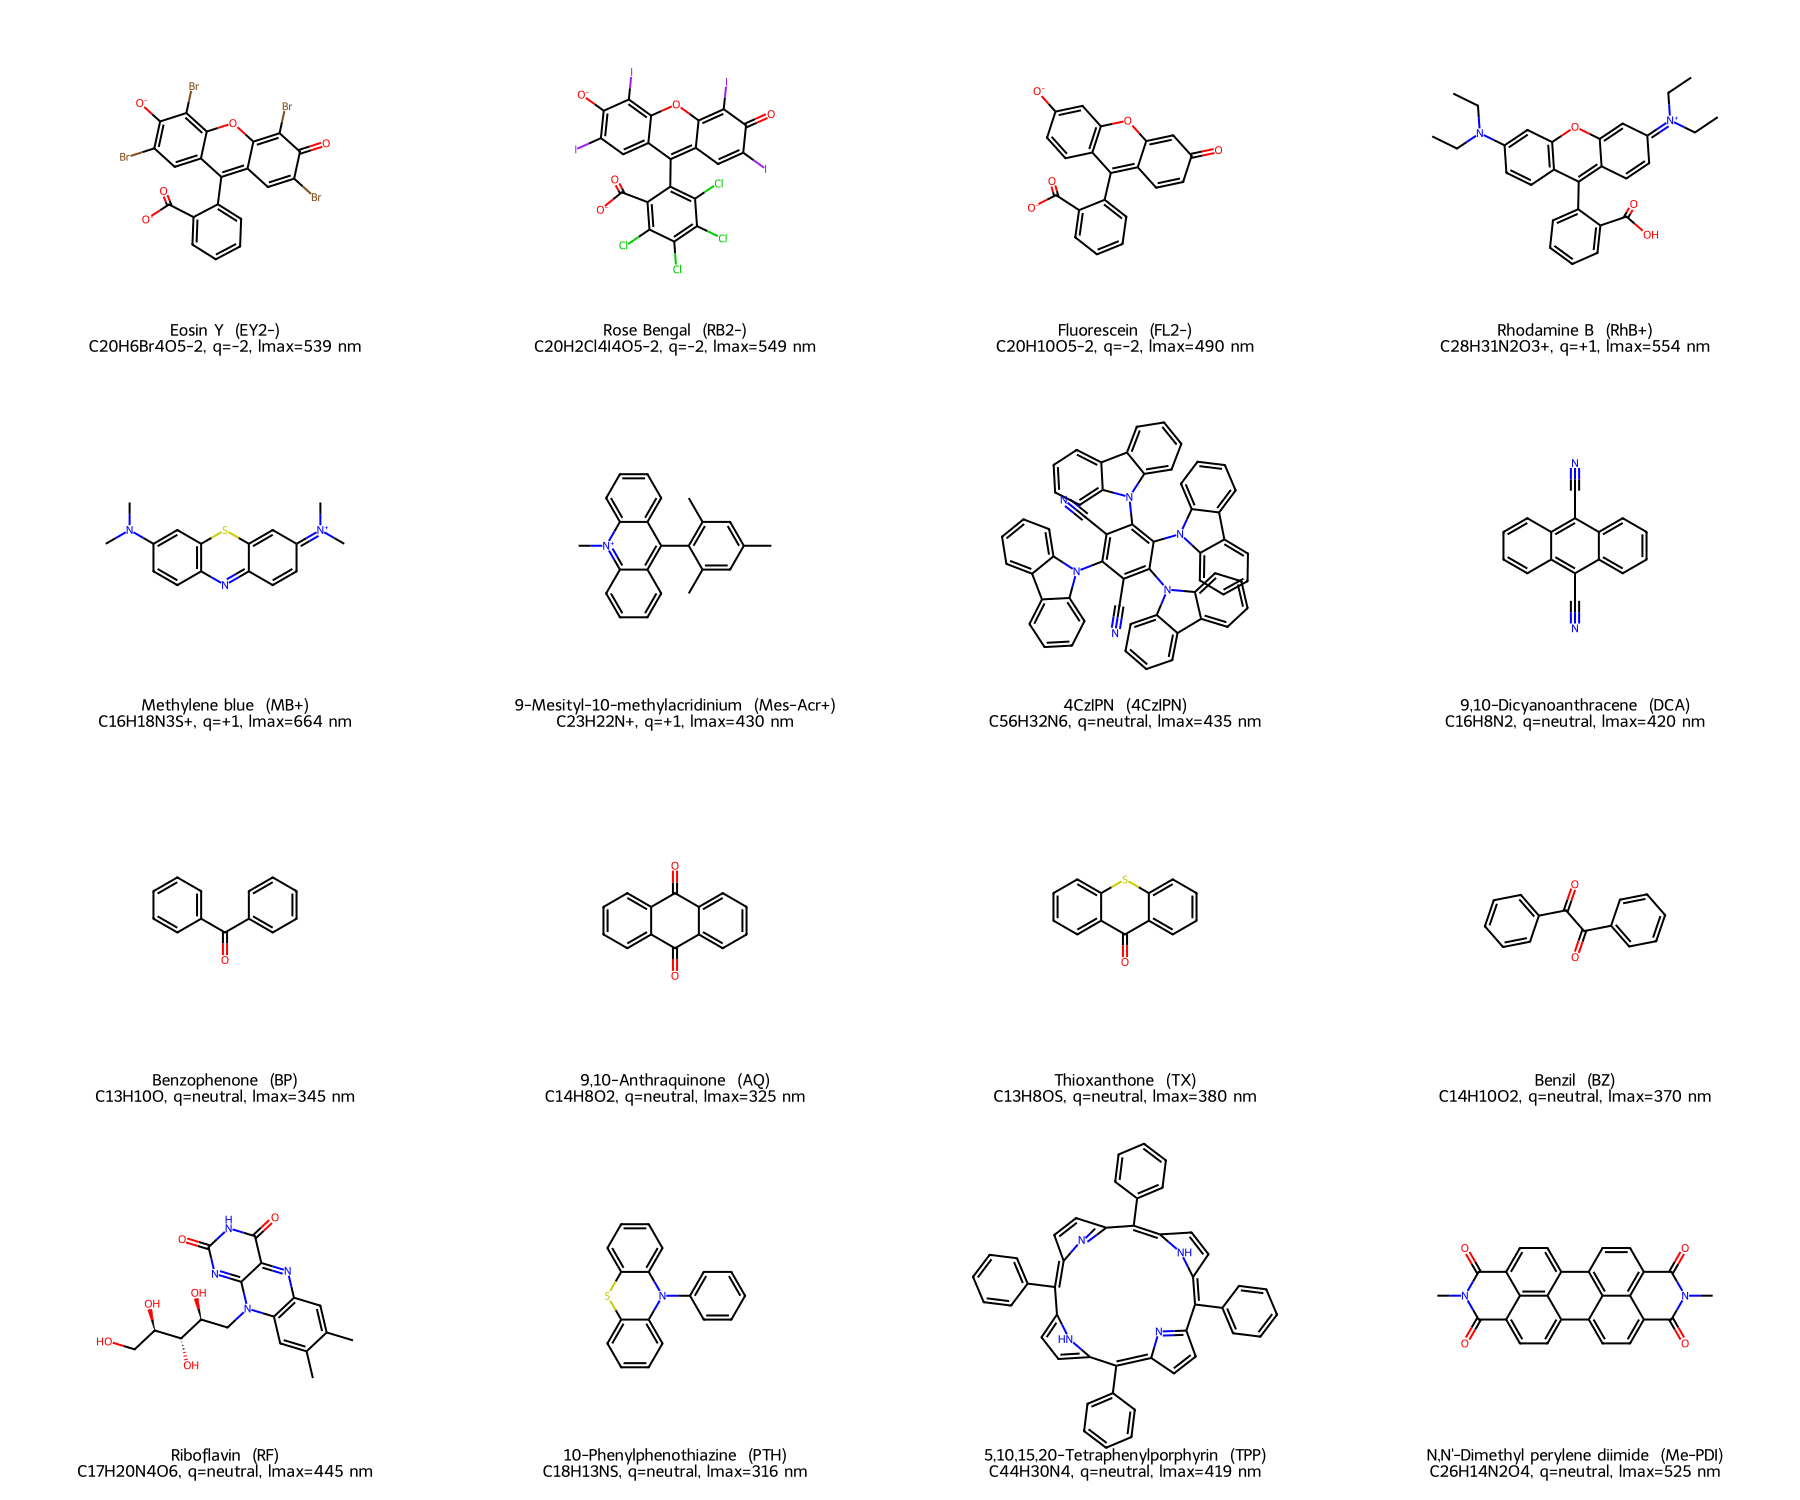
\includegraphics[width=0.82\linewidth]{organic_photocatalysts_grid.png}
\caption{The 16 molecules as encoded. Charges are part of the identity: \ce{EY^{2-}},
\ce{RB^{2-}} and \ce{FL^{2-}} are dianions; \ce{MB+}, \ce{RhB+} and Mes-Acr$^+$ are cations.}
\end{figure}

\paragraph{PubChem cross-check.} Each name was resolved against PubChem. 9 of 16 stored species
match a PubChem record exactly. For the other 7, \texttt{pubchem\_parent\_cid} points to a
\emph{related} record, and \texttt{pubchem\_cid\_relation} explains how they relate:
\begin{itemize}
  \item salts (EY, RB, RhB, MB, Mes-Acr): PubChem stores the salt; we keep only the active ion;
  \item fluorescein: PubChem's main record is the neutral lactone; we use the quinoid dianion;
  \item Me-PDI: no PubChem record; built from the parent PTCDA (CID 67191).
\end{itemize}

\begin{learn}
\textbf{Compute the species that does the chemistry.} In water at working pH, eosin~Y is a
dianion, and its colour and redox potentials belong to that dianion. The InChIKey records this
in its last letter: neutral eosin~Y ends in \texttt{-N}, the dianion in \texttt{-L} (two protons
removed). The first 14 characters, which encode the skeleton, are identical. That is why a
salt or ion can be traced back to its parent record in PubChem.
\end{learn}

\subsection{Checks before any 3D work}
For each row the script parses the SMILES (RDKit returns \texttt{None} on a syntax error; the
molecule is then skipped). It then computes formula, total charge and InChIKey from the parsed
structure and compares each with the stored value. Mismatches go into a \texttt{problems} list
instead of stopping the run, so all errors are reported at once.

\begin{caveat}
The formula and charge checks catch real typos. For example, dropping one \texttt{(Br)} from the
eosin~Y SMILES still gives a valid SMILES, but the formula becomes \ce{C20H7Br3O5^{2-}}. The
InChIKey check, however, can only catch \emph{later edits}, because the stored key was itself
generated from the same SMILES. The independent check is the PubChem comparison above.
\end{caveat}

\subsection{Multi-conformer 3D embedding}
\begin{enumerate}
  \item \texttt{AddHs}: implicit hydrogens become real atoms, so they get coordinates
  (eosin~Y: 29 $\to$ 35 atoms).
  \item \textbf{ETKDGv3} distance-geometry embedding with a fixed random seed
  (\texttt{0xF00D}). It generates 8 conformers, or 30 if the molecule has more than 3 rotatable
  bonds. Conformers within 0.5~\AA\ RMSD of each other are pruned as duplicates.
  \item Every conformer is minimised with \textbf{MMFF94s}, and the lowest-energy one is written
  to xyz with \texttt{charge=\ldots\ mult=1} in the comment line. The xyz format has no charge
  field; \texttt{read\_xyz} recovers it with the regular expression \verb|charge=(-?\d+)|.
\end{enumerate}

\begin{center}\small
\begin{tabular}{@{}lccc@{}}
\toprule
Molecule & Rotatable bonds & Conformers tried & Kept after pruning \\
\midrule
anthraquinone & 0 & 8 & 1 \\
eosin Y$^{2-}$ & 2 & 8 & 2 (mirror images, identical energy) \\
riboflavin & 9 & 30 & 18 \\
\bottomrule
\end{tabular}
\end{center}

\begin{learn}
The number of surviving conformers measures flexibility. A rigid molecule collapses to one
structure however many times you embed it. Riboflavin's ribityl chain gives 18 distinct shapes
spread over 14~kcal/mol in MMFF energy. The two eosin~Y conformers have the benzoate ring twisted
one way or the other, which is why they are exactly degenerate.
\end{learn}

\begin{figure}[h]
\centering
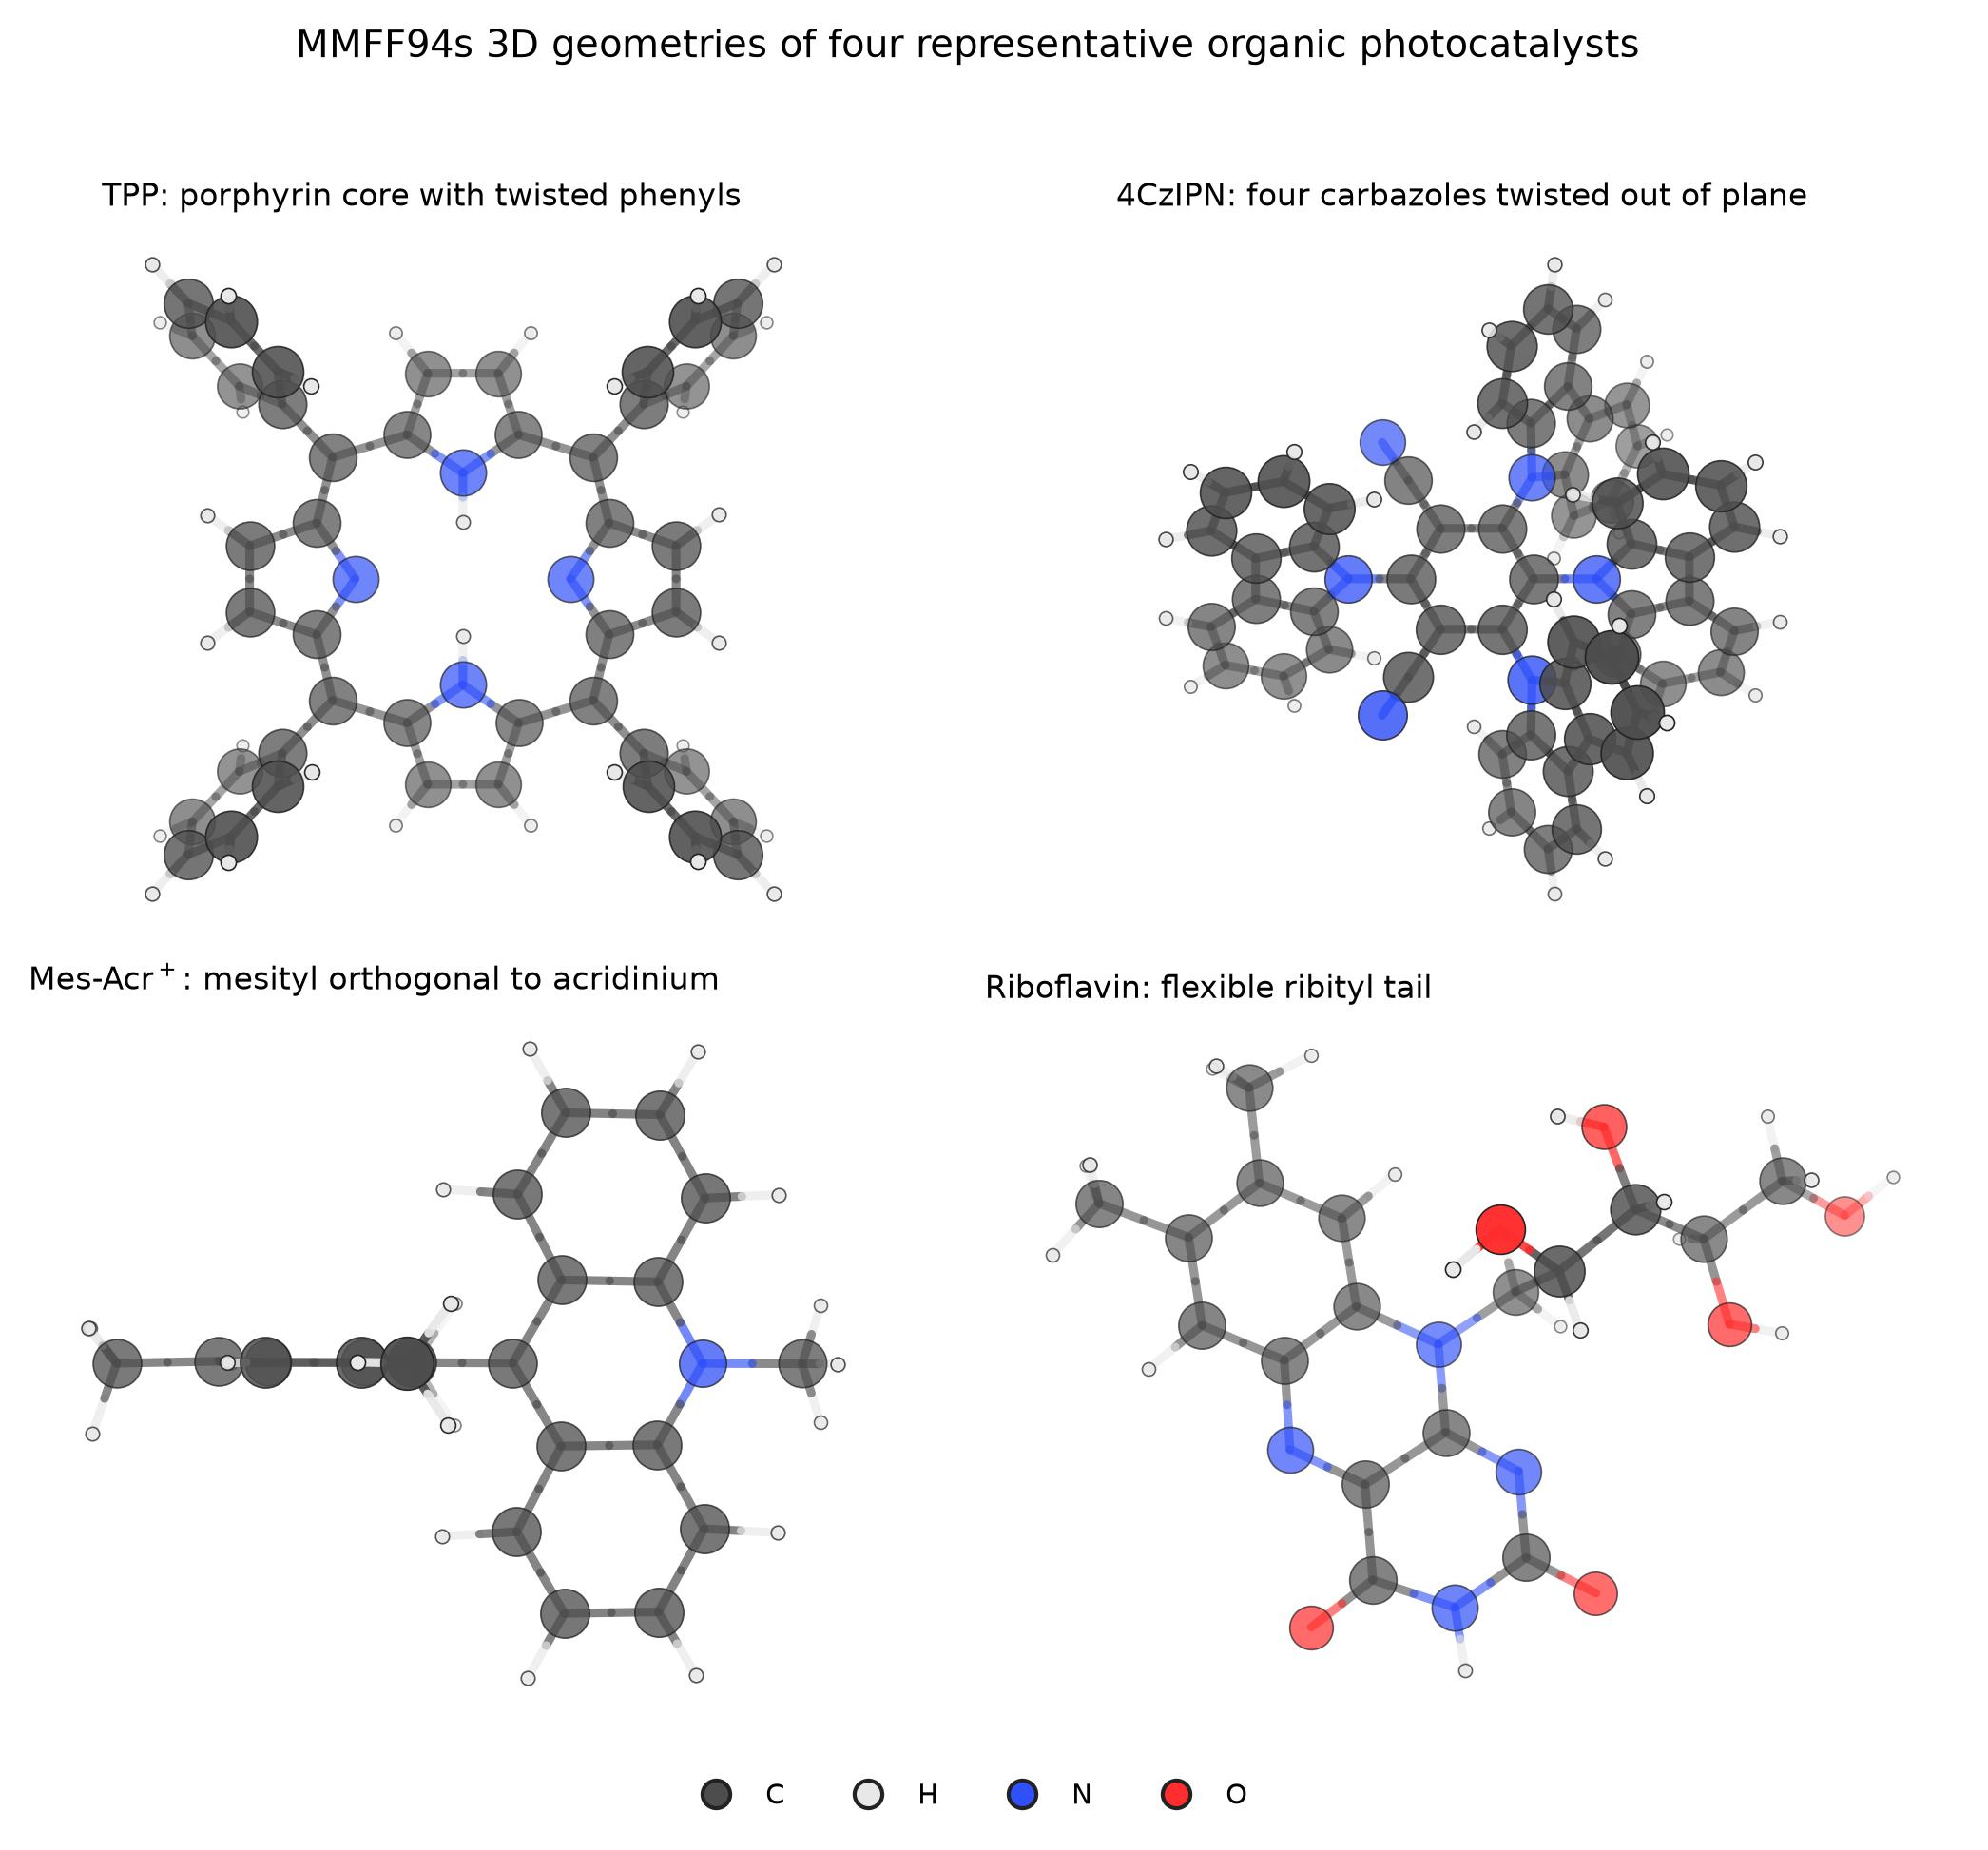
\includegraphics[width=0.72\linewidth]{structures_3d_montage.png}
\caption{MMFF94s geometries. Each feature shown is a twist that decouples two $\pi$ systems
(TPP phenyls, 4CzIPN carbazoles, Mes-Acr$^+$ mesityl) or a flexible tail (riboflavin).}
\end{figure}

%=============================================================================
\section{Step 2 --- DFT geometry optimisation}

\subsection{What the script does}
\begin{enumerate}
  \item Builds the PySCF molecule from the MMFF xyz (\texttt{build\_mol}). def2 effective core
  potentials are added automatically for elements heavier than Kr ($Z>36$), i.e.\ iodine in rose
  bengal; bromine ($Z=35$) does not need one.
  \item Runs an SCF on the MMFF geometry, which gives the reference energy $E_\text{MMFF geom}$.
  \item Optimises with \textbf{geomeTRIC}, which steps in internal coordinates (bonds, angles,
  torsions) rather than raw $x,y,z$.
  \item Runs a final SCF at the optimised geometry, then compares the two structures with a
  \textbf{Kabsch-aligned RMSD}.
\end{enumerate}

\begin{learn}
\textbf{Kabsch alignment.} Two copies of the same molecule can differ simply by being rotated or
shifted. Kabsch's algorithm first centres both copies, then finds the rotation that best
superimposes them (via a singular value decomposition of $P^\mathsf{T}Q$). Only then does it
measure the per-atom distances. Without it, an RMSD would mix real structural change with an
arbitrary orientation. The script reports RMSD over all atoms, over heavy atoms only, and the
single largest atomic displacement.
\end{learn}

\subsection{Convergence criteria: \texttt{gau} vs \texttt{flat}}
An optimisation stops when \emph{all} of its tests pass. The default (\texttt{gau},
Gaussian-like) has three kinds of test:

\begin{center}\small
\begin{tabular}{@{}lcc@{}}
\toprule
Test & \texttt{gau} & \texttt{flat} \\
\midrule
energy change per step & $10^{-6}$ Ha & $10^{-5}$ Ha \\
gradient (RMS / max) & $3\times10^{-4}$ / $4.5\times10^{-4}$ Ha/bohr & same \\
displacement (RMS / max) & $1.2\times10^{-3}$ / $1.8\times10^{-3}$ bohr & effectively off \\
\bottomrule
\end{tabular}
\end{center}

For eosin~Y, 27 \texttt{gau} steps met the gradient test, but the displacement test never
settled. The optimiser kept taking sizeable steps along very soft torsions (the benzoate twist)
at almost no cost in energy. The run was therefore resumed from its last frame with
\texttt{--criteria flat}, which keeps the same gradient thresholds but drops the displacement
test. It converged in 4 more steps. Riboflavin and rhodamine~B used \texttt{flat} from the start.

\begin{learn}
\textbf{Flat potential energy surfaces.} The gradient tells you the surface is level; the
displacement tells you the optimiser has stopped moving. On a very flat torsional surface the
gradient can be small while the atoms still wander. Relaxing the displacement test is
reasonable \emph{because} the gradient test still holds. The structure is a true stationary
point, but the exact torsion angle is poorly determined. Report it with that caveat.
\end{learn}

\subsection{Results}
\begin{center}\small
\begin{tabular}{@{}lrrrrrl@{}}
\toprule
Molecule & AO & Cycles & $\Delta E$ (kcal/mol) & RMSD$_\text{heavy}$ (\AA) & Max dev.\ (\AA) & Criteria \\
\midrule
thioxanthone & 254 & 10 & $-1.88$ & 0.030 & 0.06 & gau \\
anthraquinone & 264 & 15 & $-1.42$ & 0.019 & 0.04 & gau \\
benzophenone & 246 & 11 & $-1.27$ & 0.096 & 0.26 & gau \\
\midrule
riboflavin & 478 & 18 & $-11.13$ & 0.173 & 0.65 & flat \\
eosin Y$^{2-}$ & 508 & 31 & $-17.73$ & 0.316 & 1.30 & gau $\to$ flat \\
rhodamine B$^+$ & 617 & 20 & $-20.23$ & 0.398 & 1.27 & flat \\
\bottomrule
\end{tabular}
\end{center}
\noindent $\Delta E = E(\text{DFT-optimised}) - E(\text{MMFF geometry})$, both at the same DFT
level. Wall times: rhodamine~B 68\,073~s ($\approx$19~h), riboflavin 5\,547~s ($\approx$1.5~h);
eosin~Y's recorded 711~s covers only the 4-step resume.

\begin{finding}
The earlier conclusion ``MMFF is good enough, so skip DFT for the other 13'' does not hold. It
was based on three rigid molecules. The flexible and charged dyes moved roughly 6--13 times more than the rigid
ones (heavy-atom RMSD 0.17--0.40 vs 0.02--0.03~\AA) and dropped 11--20~kcal/mol in energy.
\end{finding}

\paragraph{What actually moved.} I aligned each MMFF and DFT pair and listed the atoms that moved
most:
\begin{itemize}
  \item \textbf{Eosin Y$^{2-}$}: the largest mover is a carboxylate oxygen (1.30~\AA). The
  ring--ring twist changed from \ang{98.6} to \ang{86.1}.
  \item \textbf{Rhodamine B$^+$}: again a carboxylic-acid oxygen (1.27~\AA), with the ring--ring
  twist almost unchanged ($-\ang{84.9}\to-\ang{88.9}$). The next movers are ethyl hydrogens.
  \item \textbf{Riboflavin}: hydroxyl hydrogens and oxygens of the ribityl chain (up to
  0.65~\AA). This looks like a hydrogen-bond rearrangement.
\end{itemize}
So the large RMSDs come mainly from the \textbf{carboxyl groups and side chains rotating}, not
from the chromophore cores. A likely reason is that MMFF minimised these ions without any solvent,
while the DFT run used ddCOSMO water. A bare \ce{-COO-} group in vacuum and a solvated one prefer
different orientations. Because the HOMO and LUMO of these dyes sit on the cores, the orbital
energies may change much less than the RMSD suggests. Step~5 exists to test exactly this
(Section~6).

\begin{figure}[h]
\centering
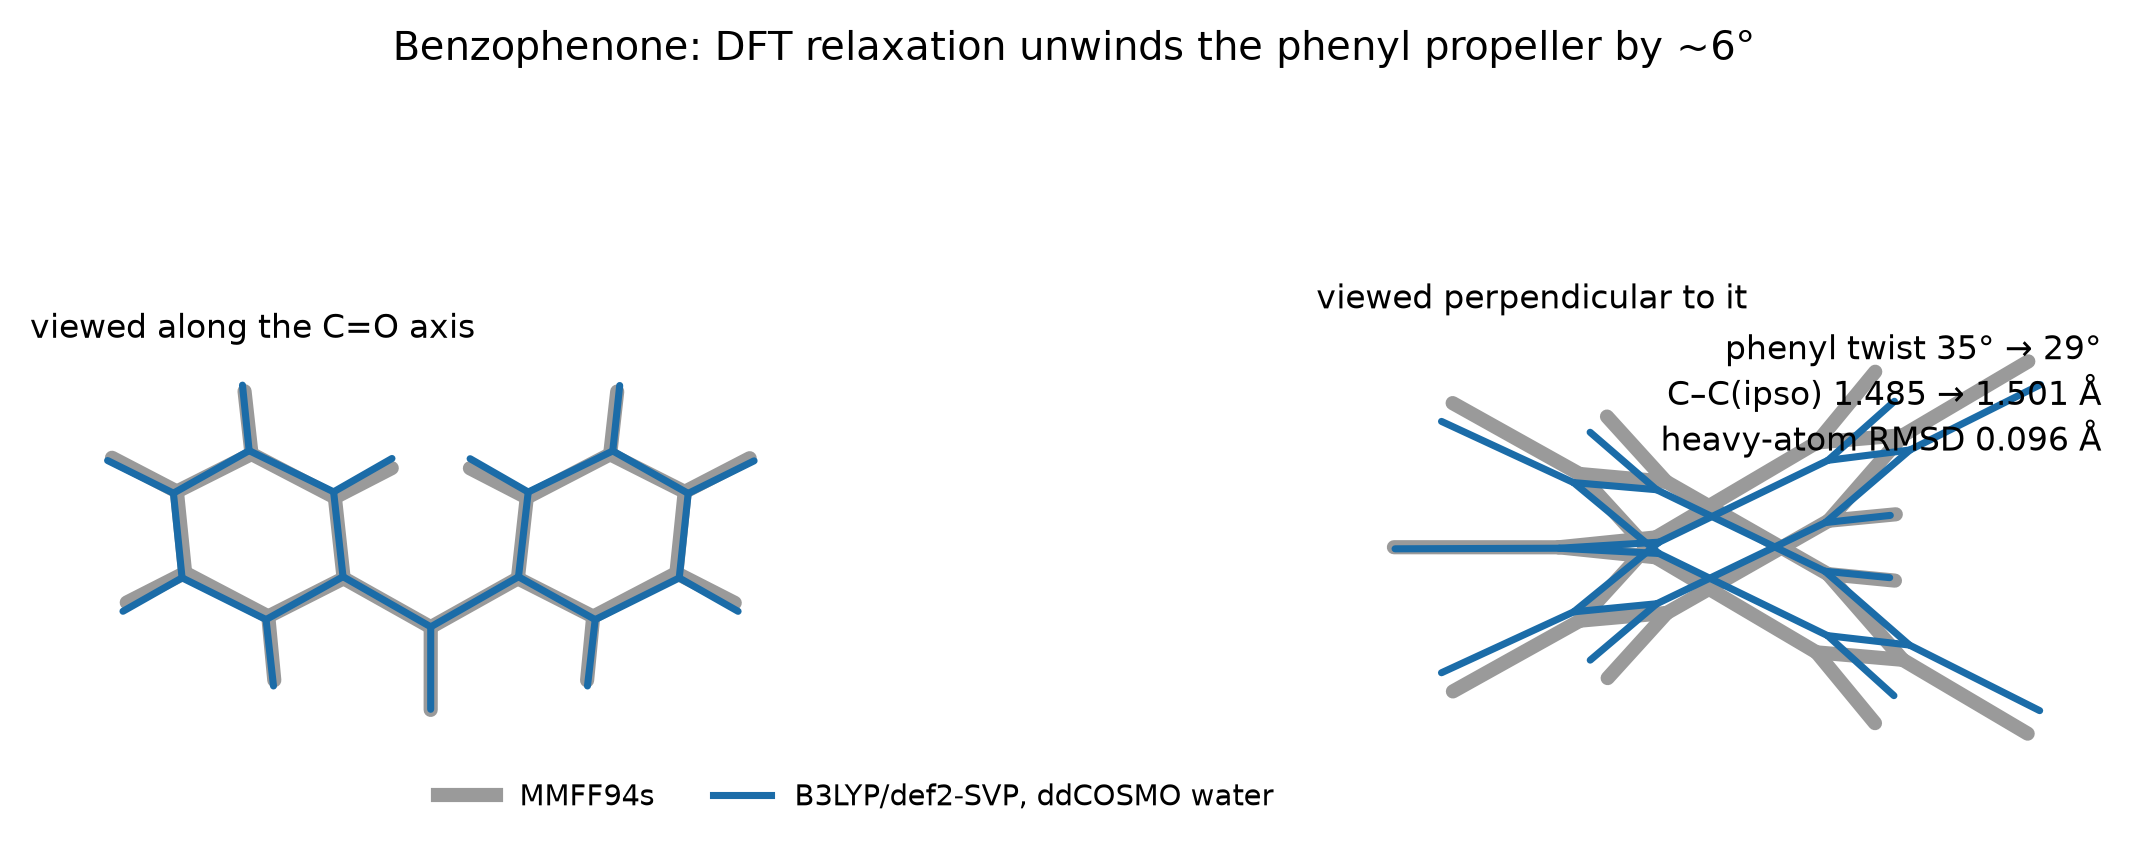
\includegraphics[width=0.9\linewidth]{geomopt_overlay_benzophenone.png}
\caption{Benzophenone, MMFF94s (grey) vs DFT (blue): the change is invisible along C=O and
obvious from the side. Always look from two directions.}
\end{figure}

%=============================================================================
\section{Step 3 --- Frontier orbital energies}

A single point on each molecule's best available geometry: the DFT-optimised one if it exists,
otherwise the MMFF one. The column \texttt{geom\_source} records which was used. If the SCF
fails to converge, the script retries with a second-order (Newton) solver. All 16 converged.

\begin{figure}[h]
\centering
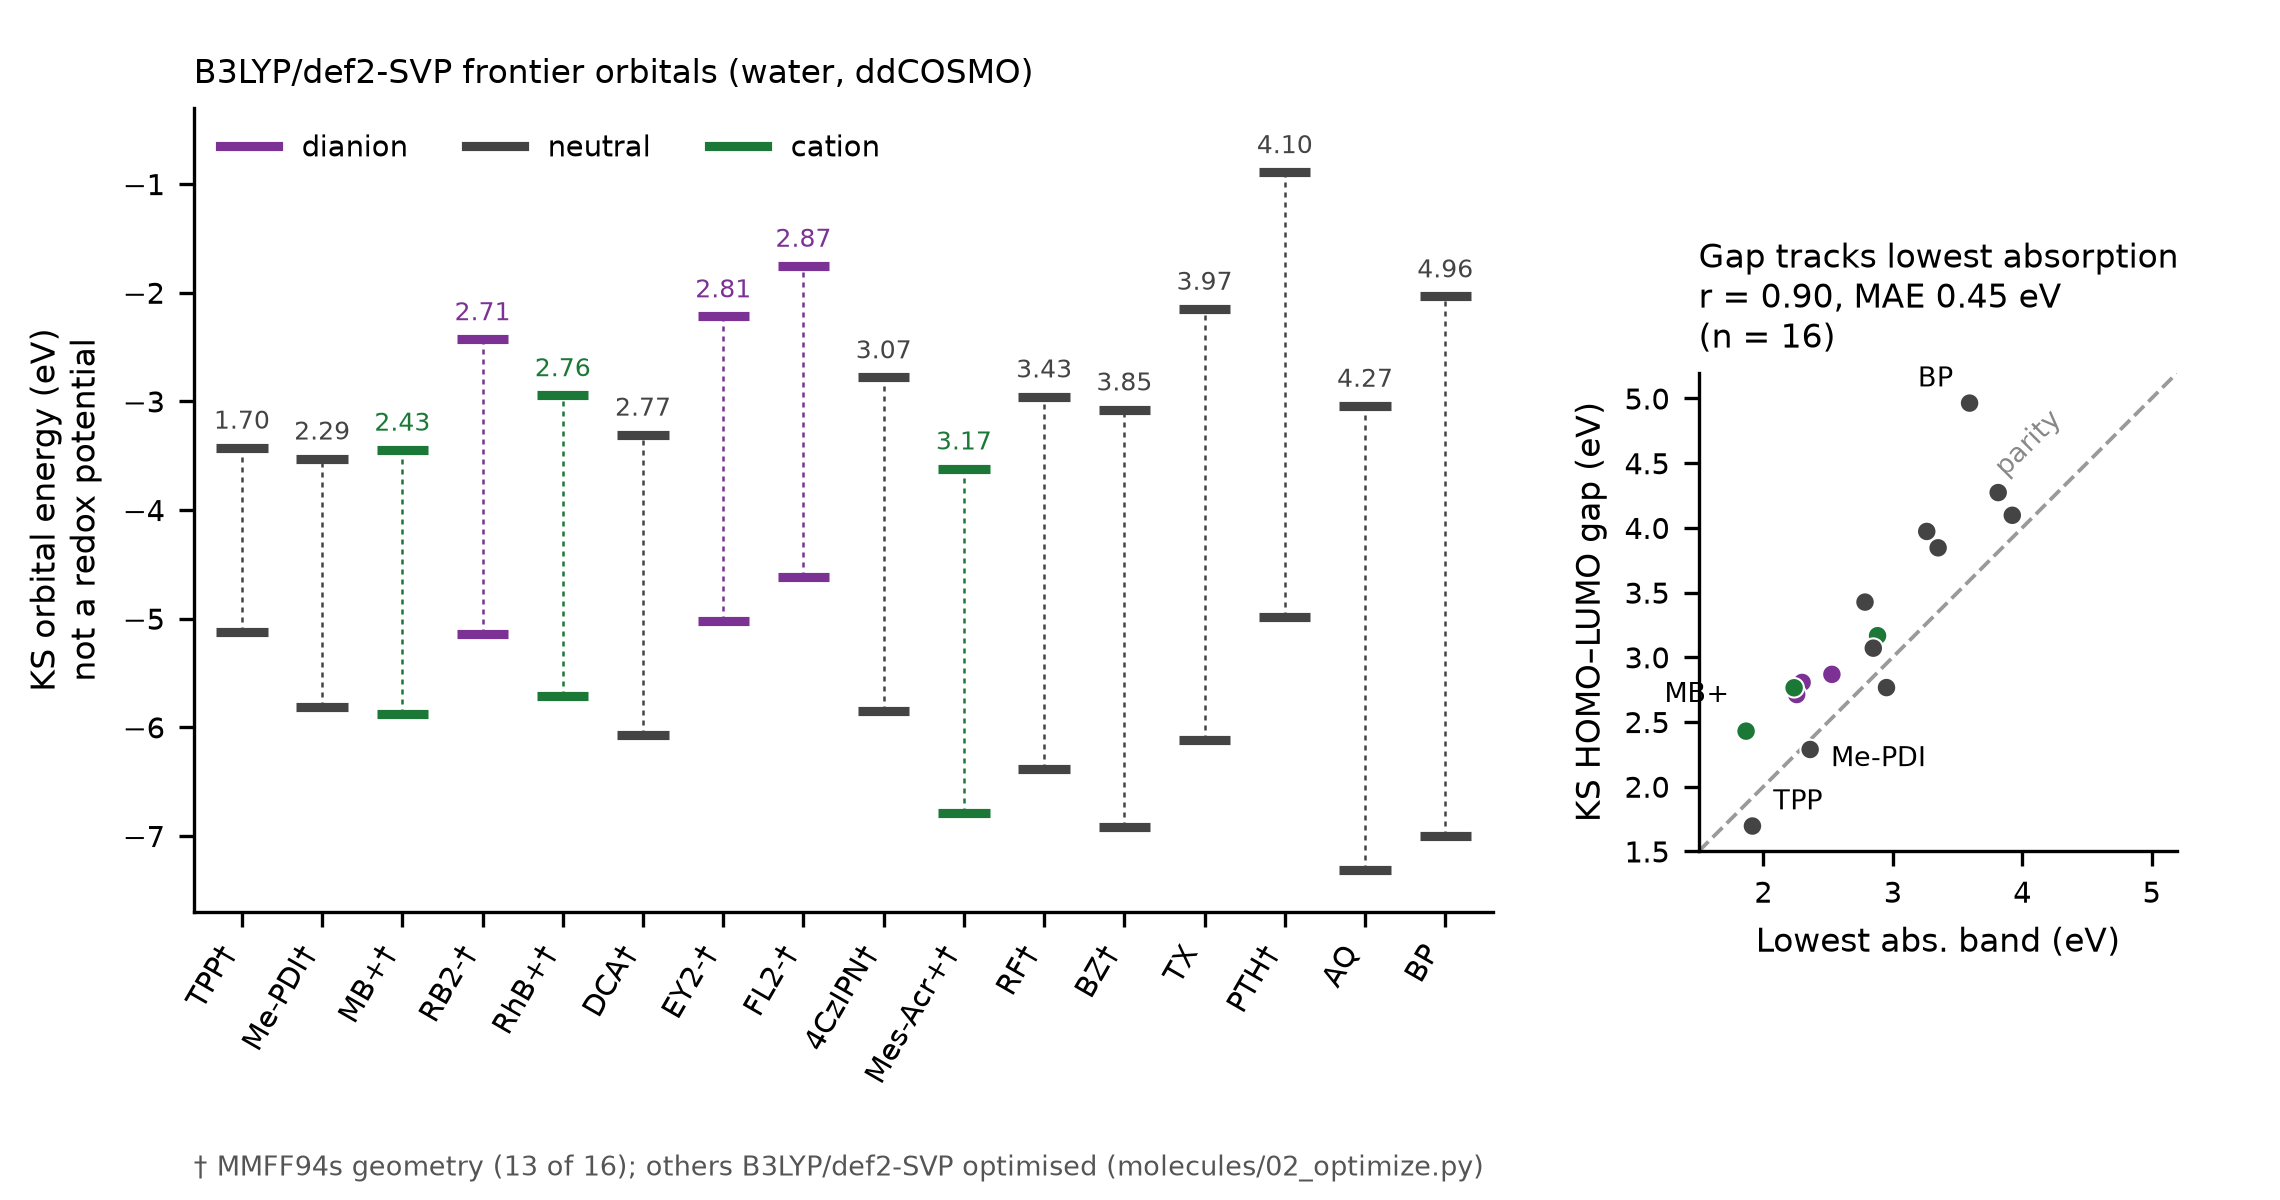
\includegraphics[width=\linewidth]{homo_lumo_diagram.png}
\caption{Current diagram. Compared with the first version, the H$^+$/H$_2$ and O$_2$/H$_2$O lines
were removed, the axis now says ``not a redox potential'', and $\dagger$ marks the 13 molecules
still on MMFF geometry.}
\end{figure}

\begin{center}\small
\begin{tabular}{@{}lrrrrl@{}}
\toprule
PC & HOMO (eV) & LUMO (eV) & Gap (eV) & Lowest abs.\ (eV) & Geometry \\
\midrule
TPP & $-5.12$ & $-3.43$ & 1.70 & 1.92 & MMFF \\
Me-PDI & $-5.81$ & $-3.53$ & 2.29 & 2.36 & MMFF \\
MB$^+$ & $-5.87$ & $-3.45$ & 2.43 & 1.87 & MMFF \\
RB$^{2-}$ & $-5.14$ & $-2.43$ & 2.71 & 2.26 & MMFF \\
RhB$^+$ & $-5.71$ & $-2.94$ & 2.76 & 2.24 & MMFF$^\ast$ \\
DCA & $-6.07$ & $-3.31$ & 2.77 & 2.95 & MMFF \\
EY$^{2-}$ & $-5.02$ & $-2.22$ & 2.81 & 2.30 & MMFF$^\ast$ \\
FL$^{2-}$ & $-4.62$ & $-1.75$ & 2.87 & 2.53 & MMFF \\
4CzIPN & $-5.85$ & $-2.78$ & 3.07 & 2.85 & MMFF \\
Mes-Acr$^+$ & $-6.79$ & $-3.62$ & 3.17 & 2.88 & MMFF \\
RF & $-6.38$ & $-2.96$ & 3.43 & 2.79 & MMFF$^\ast$ \\
BZ & $-6.92$ & $-3.08$ & 3.85 & 3.35 & MMFF \\
TX & $-6.12$ & $-2.15$ & 3.97 & 3.26 & DFT \\
PTH & $-4.99$ & $-0.89$ & 4.10 & 3.92 & MMFF \\
AQ & $-7.31$ & $-3.04$ & 4.27 & 3.82 & DFT \\
BP & $-7.00$ & $-2.03$ & 4.96 & 3.59 & DFT \\
\bottomrule
\end{tabular}

\smallskip
{\footnotesize $^\ast$ a DFT geometry now exists, but step~3 has not been rerun on it.}
\end{center}

\begin{finding}
The Kohn--Sham gap tracks the lowest experimental absorption band ($r=0.90$, MAE 0.45~eV,
$n=16$), and is larger than it for 13 of the 16. The largest outlier is benzophenone
(+1.37~eV), whose weak lowest band is n$\to\pi^*$. TPP is compared against its Q$_x$(0,0) band
(647~nm), not the Soret band, which is S$_2$.
\end{finding}

\begin{learn}
\textbf{Three gaps that are not the same thing.}
\begin{itemize}[leftmargin=*]
  \item \emph{KS HOMO--LUMO gap}: a difference of orbital energies from one ground-state
  calculation.
  \item \emph{Fundamental gap} = IE $-$ EA: needs calculations on the cation and anion. For
  benzene, B3LYP's $-\varepsilon_\text{HOMO}$ was 6.97~eV against an experimental IE of 9.24~eV.
  \item \emph{Optical gap}: the lowest excitation, which includes the electron--hole attraction.
  It needs TDDFT.
\end{itemize}
A good correlation with absorption says the \emph{trend} is captured, not that the absolute values
mean anything. This is why the redox lines were removed from the diagram.
\end{learn}

%=============================================================================
\section{Step 4 --- Where the orbitals live}

For Mes-Acr$^+$ and eosin~Y$^{2-}$, the script writes cube files for HOMO$-2$ to LUMO$+1$ (about
4.5~MB each, git-ignored). It then measures how much of each orbital sits on a ``core'' fragment,
which is defined by a SMARTS pattern. The measure is the Mulliken population of orbital
$\phi_k$ on the fragment's atoms:
\[
  p_k(\text{core}) = \sum_{\mu \in \text{core}} c_{\mu k}\,(\mathbf{S}\mathbf{c}_k)_\mu ,
\]
where $c_{\mu k}$ are the MO coefficients and $\mathbf{S}$ is the AO overlap matrix. Summed over
all atoms this gives exactly 1.

\begin{center}\small
\begin{tabular}{@{}llrl@{}}
\toprule
Molecule & Orbital & $E$ (eV) & Localisation \\
\midrule
eosin Y$^{2-}$ & HOMO & $-5.02$ & 91\% xanthene core \\
 & LUMO & $-2.22$ & 97\% xanthene core \\
 & HOMO$-1$, HOMO$-2$ & $-5.34$, $-5.83$ & 88\%, 84\% benzoate \\
Mes-Acr$^+$ & HOMO$-2$ & $-6.80$ & $>$99\% mesityl \\
 & HOMO$-1$ & $-6.79$ & 96\% mesityl \\
 & HOMO & $-6.79$ & 99\% acridinium \\
 & LUMO & $-3.62$ & 98\% acridinium \\
\bottomrule
\end{tabular}
\end{center}

\begin{figure}[h]
\centering
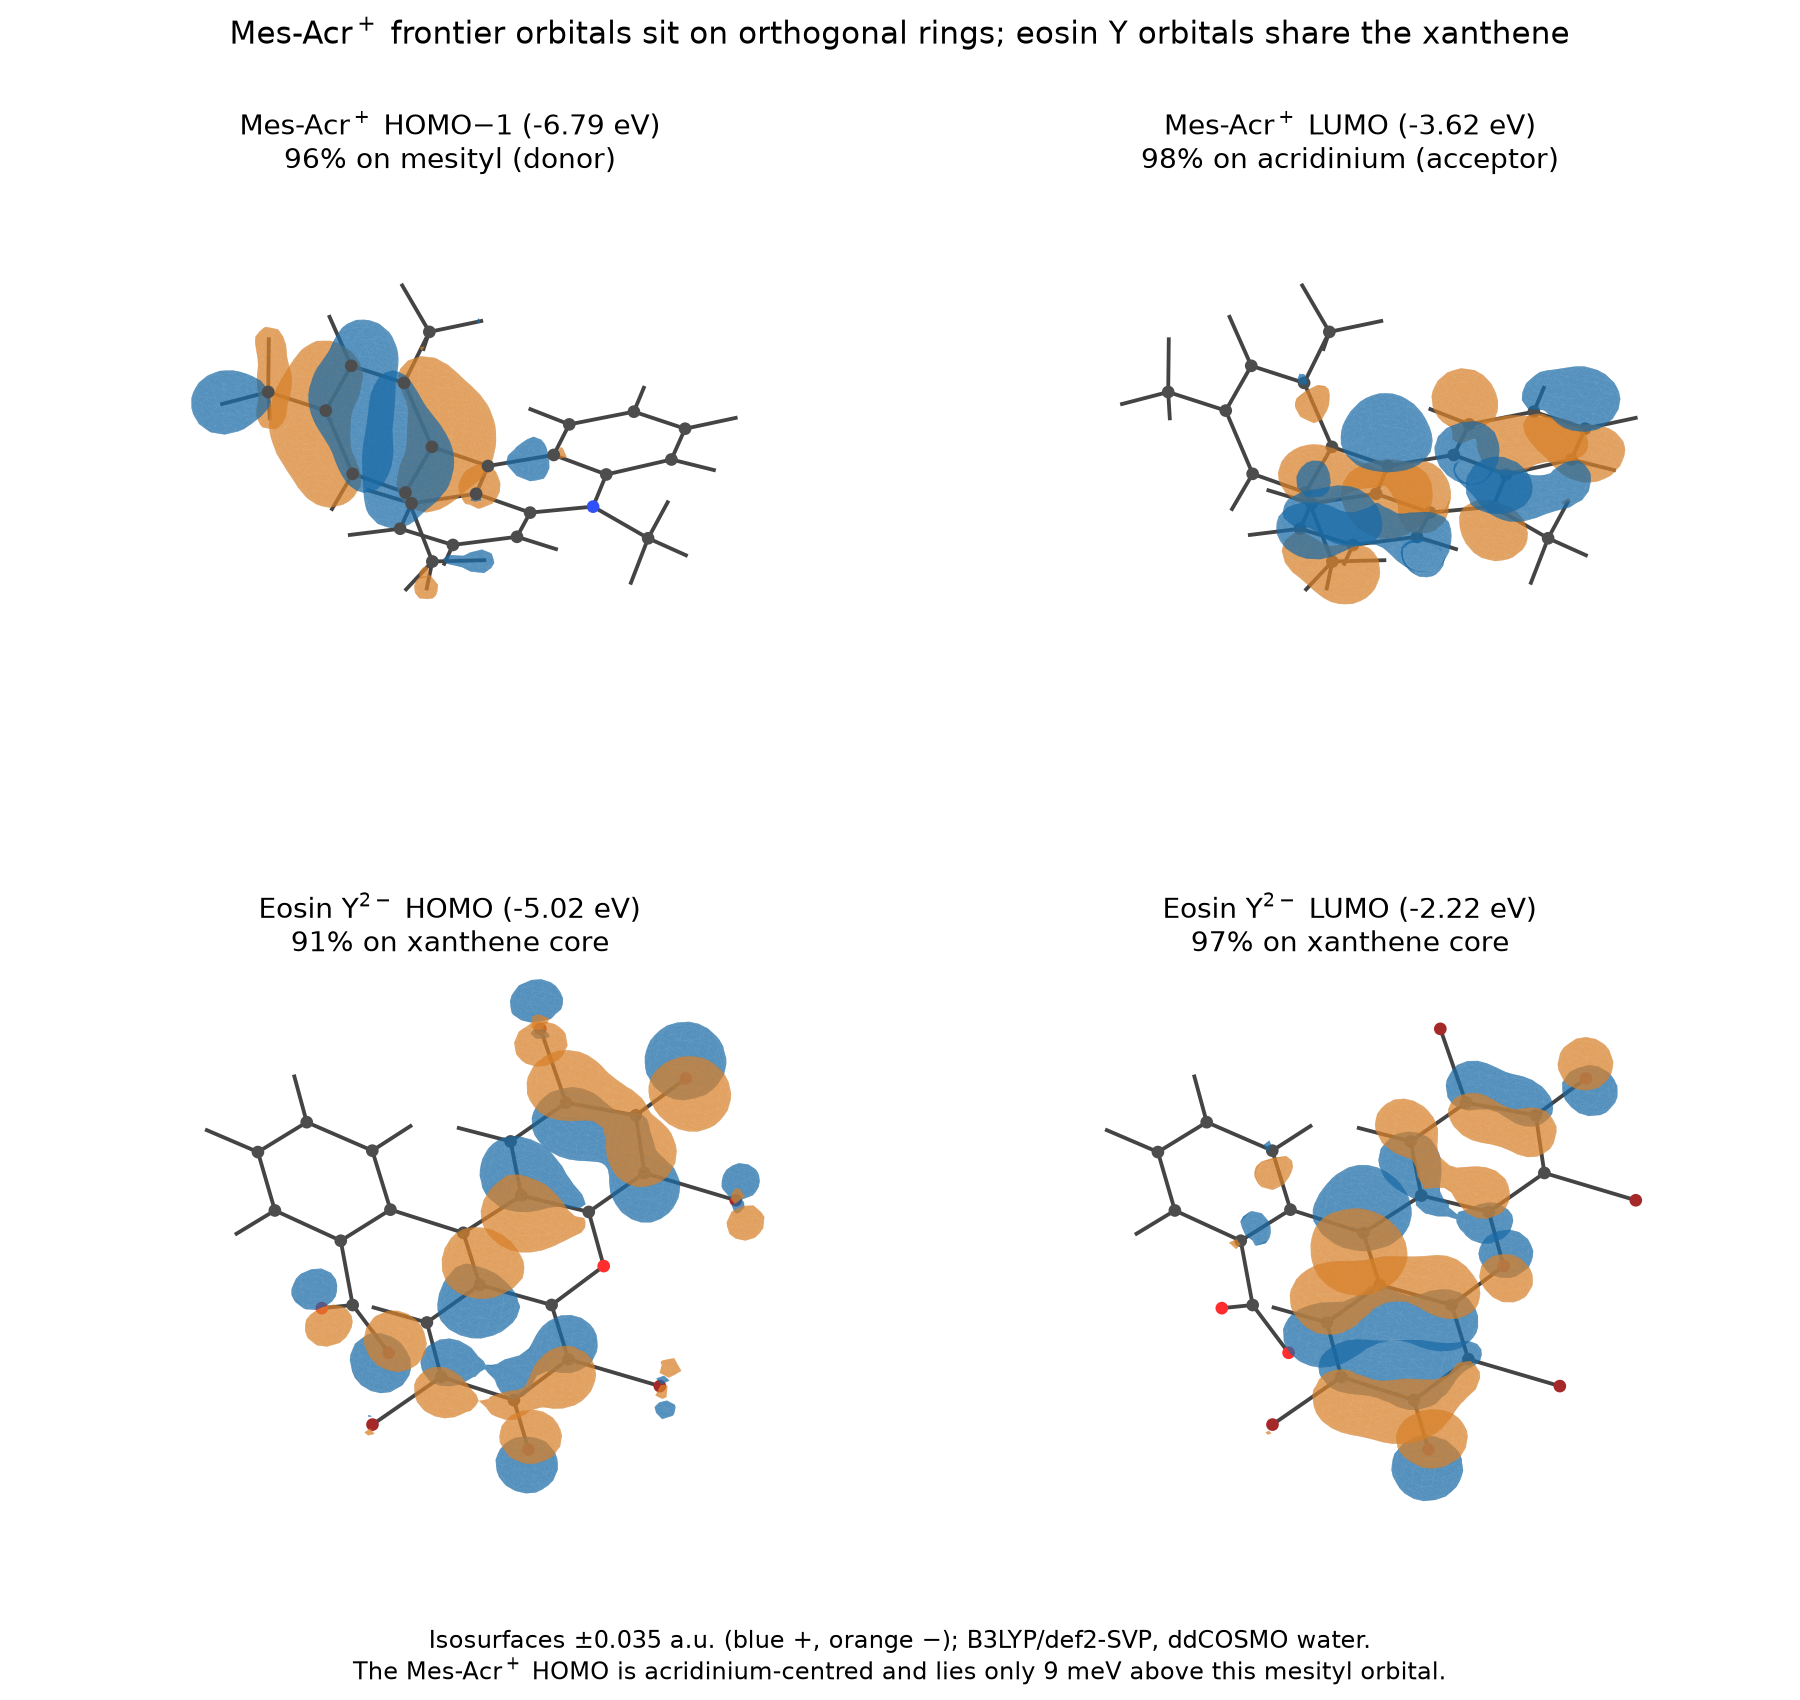
\includegraphics[width=0.62\linewidth]{frontier_orbitals_isosurfaces.png}
\caption{Isosurfaces at $\pm0.035$~a.u., rendered by marching cubes in matplotlib (schematic:
matplotlib only approximates which surface is in front).}
\end{figure}

\begin{finding}
Eosin~Y's lowest excitation is \emph{local} ($\pi\to\pi^*$ on the xanthene). In Mes-Acr$^+$,
donor (mesityl) and acceptor (acridinium) orbitals sit on two orthogonal rings, which gives
\emph{charge-transfer} character. This is the orbital-level picture of the 3D twist in
Section~2.3. The top three occupied orbitals of Mes-Acr$^+$ lie within 13~meV of each other, so
which one is labelled ``HOMO'' is not meaningful at this level of theory.
\end{finding}

\begin{caveat}
Mulliken populations depend on the basis set. Use them for qualitative statements (91\% vs 10\%),
not for small differences. The eosin~Y orbitals in this step were computed on the MMFF geometry,
before its DFT optimisation existed.
\end{caveat}

%=============================================================================
\section{Step 5 --- Does the geometry matter for the orbitals? (new, not yet run)}

\texttt{05\_geometry\_check.py} answers the question raised by Section~3.3. For every molecule
with a DFT geometry, it reruns the step-3 single point on the \emph{MMFF} geometry and compares
it with the step-3 result on the \emph{DFT} geometry. It writes the shifts
$\Delta$HOMO, $\Delta$LUMO and $\Delta$gap (DFT minus MMFF) next to the RMSD and $\Delta E$ for each
molecule.

\begin{caveat}
\textbf{It cannot produce useful output yet.} The script deliberately skips any molecule whose
step-3 entry was not computed on the DFT geometry (\texttt{geom\_source != "xyz\_opt"}). That is
currently true for eosin~Y, riboflavin and rhodamine~B: \texttt{frontier\_orbitals.csv} was last
written on 18 Oct at 14:33, before any of their optimisations finished. The order to run is:
\begin{verbatim}
python molecules/03_frontier.py --only eosinY riboflavin rhodamineB
python molecules/05_geometry_check.py
\end{verbatim}
The three rigid molecules will then show the baseline (expected to be near zero). The three
flexible ones will show whether rotating the carboxyl groups and side chains moves the frontier
orbitals.
\end{caveat}

\noindent\textbf{How to read the answer.} If $|\Delta\text{gap}|$ is small compared with the
0.45~eV MAE against experiment, MMFF geometries are adequate \emph{for this property}, and the
remaining 10 molecules need not be optimised. If it is comparable, every molecule needs DFT
geometries before the orbital table can be trusted.

%=============================================================================
\section{Infrastructure worth understanding}

\begin{itemize}
  \item \textbf{The dispersion workaround} (\texttt{utils/common.py}). On the Mac,
  \texttt{pyscf-dispersion} fails to load its compiled library. Because PySCF tries to import
  it, \texttt{import pyscf} itself crashed. The helper attempts the import, catches the
  \texttt{TypeError}, deletes the half-loaded PySCF modules from \texttt{sys.modules}, registers
  an empty placeholder module called \texttt{pyscf.dispersion}, and re-imports. PySCF then takes
  its own ``no D3 available'' path, and everything except dispersion works. This is why every
  script must import \texttt{utils.common} before \texttt{pyscf}, and why no result includes D3.
  \item \textbf{Density fitting} (\texttt{.density\_fit()}) approximates the four-index electron
  repulsion integrals with an auxiliary basis. It is much faster at a very small accuracy cost,
  and is what made the 617-function rhodamine~B optimisation feasible.
  \item \textbf{ddCOSMO} places the molecule in a cavity inside a dielectric continuum
  ($\varepsilon=78.36$ for water). It matters most for the ions: a bare dianion in vacuum barely
  binds its extra electrons.
  \item \textbf{Provenance}: every xyz comment line records method, criteria, convergence and
  energy. Every CSV row records level of theory, geometry source and wall time.
\end{itemize}

%=============================================================================
\section{Status board}

\begin{center}\small
\begin{tabularx}{\linewidth}{@{}lX@{}}
\toprule
\multicolumn{2}{@{}l}{\textbf{Done}} \\
\midrule
Catalogue & 16 organic photocatalysts, PubChem-checked, charge states documented \\
3D structures & Multi-conformer MMFF94s geometries for all 16; HTML viewer \\
DFT geometries & 6 of 16 (3 rigid, 3 flexible/charged) \\
Orbitals & HOMO/LUMO for all 16; localisation for EY$^{2-}$ and Mes-Acr$^+$ \\
Figure fixes & Redox lines removed; MMFF-geometry molecules marked \\
\midrule
\multicolumn{2}{@{}l}{\textbf{Outstanding}} \\
\midrule
Rerun step 3 & for EY, RF, RhB on their DFT geometries; then run step 5 \\
Remaining geometries & 10 molecules, depending on the step-5 result \\
TDDFT & not started; needed for any comparison with absorption energies \\
CT functional & CAM-B3LYP or $\omega$B97X-D for Mes-Acr$^+$ and 4CzIPN \\
Dispersion & D3 unavailable on the Mac; affects stacked or twisted structures \\
Solids (Week 2) & \texttt{solids/qe/} is empty; Materials Project and periodic DFT not started \\
\midrule
\multicolumn{2}{@{}l}{\textbf{Stale documents}} \\
\midrule
\texttt{README.md}, \texttt{REPORT.md} & last updated 17 Oct; don't mention the three new
optimisations, the \texttt{flat} criteria, step 5, or the diagram changes \\
\texttt{data/catalysts.csv} & the original 29-entry list, superseded by
\texttt{organic\_photocatalysts.csv} but still present \\
\bottomrule
\end{tabularx}
\end{center}

%=============================================================================
\section{Check yourself before meeting your PI}

\begin{enumerate}
  \item Why is eosin~Y computed as \ce{EY^{2-}}, and how does the InChIKey show it?
  \item Why does eosin~Y keep 2 conformers and riboflavin 18 after pruning?
  \item What does Kabsch alignment remove before an RMSD is computed?
  \item Why did eosin~Y need the \texttt{flat} criteria, and why is that still a valid minimum?
  \item The three flexible dyes have RMSDs of 0.17--0.40~\AA. Which atoms moved, and why might
  that matter less for the orbitals than the RMSD suggests?
  \item What exactly does step~5 compare, and why does it currently skip every flexible
  molecule?
  \item Name three different ``gaps'' and the calculation each one needs.
  \item Why is ``the HOMO of Mes-Acr$^+$'' not a meaningful label here?
  \item What does the \texttt{pyscf.dispersion} workaround do, and what does it cost us?
\end{enumerate}

\section{Questions worth raising with your PI}
\begin{itemize}
  \item Is a geometry sensitivity below about 0.1~eV in the gap enough to keep MMFF geometries for
  the rest, or does the group want all molecules DFT-optimised regardless?
  \item For TDDFT, which functional does the group prefer (B3LYP for comparability,
  CAM-B3LYP/$\omega$B97X-D for charge-transfer dyes)?
  \item Is there cluster time for the larger molecules? Rhodamine~B alone took about 19~h.
  \item Should Week~2 (solids) start now in parallel, or after TDDFT?
\end{itemize}

\end{document}
